\chapter{Links}
\begin{figure}
    \centering
    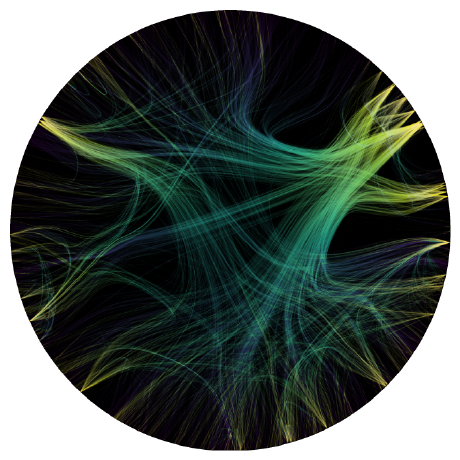
\includegraphics[width=.6\textwidth]{power/figures/metaunityplaceholder.png}
    \caption{A visualisation of the Unity game engine, produced using the Unity game engine. TODO: explanation of hierarchy and labels around perimeter. Also move this to the start of the chapter}
    \label{fig:metaunity}
\end{figure}
The previous chapter of was an exploration of how to position the nodes of a graph, and the natural question to then ask is how to deal with the only remaining component: the links. However this question is seemingly redundant at first, as the obvious answer is to simply draw straight lines between nodes with edges between them. While this by no means a poor choice, and is exactly how all node-link diagrams have been drawn thus far, this chapter will explore the possibility of drawing links using curves instead.

\section{Background}
The curving of links in the context of a node-link diagram is known as \textit{edge bundling}. It is a technique that has been developed because many networks, when processed through a standard force-directed layout, result in a seemingly random layout with no discernable structure. See Figure~\ref{TODO} for an example. The similarity of such layouts to tangled piles of hair has led to them being colloquially termed \textit{hairballs}.

Unfortunately this is not an easily solved problem, because the \textit{curse of dimensionality} \cite{Friedman2001} means that most of these networks simply cannot be accurately represented in two dimensions, and the likelihood of this problem only rises as the size of any network increases. This is all even if there is a clear underlying structure to these networks, lying beyond the reach of the standard layout algorithm.
Edge bundling attempts to alleviate this issue by introducing a trade-off---the ability to follow individual links is sacrificed for better representation of global structure, by allowing links to overlap.

This is analogous to organising the wires in a computer system by tying groups of wires together that share similar endpoints. A simple example of this is illustrated in Figure~\ref{TODO}, where the compromise between being able to follow links showing global structure is clearly visible.

The literature is rich with various different methods for performing this bundling, dating all the way back to the 1800s with the flow maps of Minard \cite{Minard1862} or Sankey diagrams \cite{Sankey1896}.
More modern algorithms for performing bundling automatically include multilevel agglomerative edge bundling (MINGLE) by Gansner et al.~\cite{Gansner2011} which greedily merges pairs of links at a time by selecting the pairs that minimise a cost function based on the amount of `ink' used to draw links. A more complex cost function is used in metro-style bundling by Pupyrev et al.~\cite{Pupyrev2016}, which is based on multiple criteria including ink, individual edge lengths and node separations. 
The same premise behind force-directed node layout is also used in force-directed edge bundling by Holten and van Wijk \cite{Holten2009}, which bundles links by defining forces between adjacent links instead of nodes. As shown previously in Section~\ref{sec:force_background}, force-based methods are in fact gradient descent optimisation methods where the gradient is defined before the cost function itself, and this edge bundling technique is no different.

Another effective approach is \emph{kernel density estimation} by Hurter et al.~\cite{Hurter2012}, who iteratively apply a convolutional filter over a density map of links in an already rendered diagram. This method belongs to the subfield of image-based bundling methods \cite{Telea2018,TODO}. A diverse gallery of edge bundling algorithms applied to the same dataset can be see in the review of Luilier et al.~\cite[Fig.~4]{Luilier2017}.
However all of the aforementioned methods share a key similarity: they apply bundling upon the assumption that node positions are predetermined and will not be moved. This is perfectly fine and even desirable in many common use cases where nodes have a predefined location, such as geographical maps, but methods such as force-directed layouts were never designed to place similar edges in parallel. In fact, the angular resolution of edges sharing nodes is sometimes used as part of the optimised cost function \cite{Argyriou2010}) and so common layout methods usually do not help, if not worsen, the bundling quality of their visualisations.

This is why one of the most powerful network visualisation techniques is method known as \emph{hierarchical edge bundling}, published by Holten in 2006 \cite{Holten2006}, recognised by a `Test of Time' award at the conference IEEE VIS in 2016.
An example of this technique in action can be seen in Figure~\ref{fig:metaunity}, which contains this visualisation applied to the source code of the Unity game engine.
The reason behind its effectiveness is that it uses extra metadata in order to inform the nature of the bundling; specifically every vertex in the visualised graph also exists as a leaf vertex in a hierarchical tree. As an example, the common and effective use case used in Figure~\ref{fig:metaunity} is to visualise the call graph of a piece of software. Each function is a vertex, and is connected by an edge to any other function that calls it. The metadata in this case is the hierarchy of folders and source files within.

The trick to the bundling is as follows: the hierarchy, not the call graph itself, is first layed out as a tree. Then, since this tree contains extra nodes to represent the folders and source files, these extra nodes are erased from the final visualisation. However their coordinates are instead used as an auxiliary routing graph (ARG) through which the call graph edges are routed through.
More precisely, this process of routing involves taking every edge in the call graph, and rendering each one using a spline curve whose control points consist of a path through the ARG. The precise definition of this spline is important, and will be further elaborated upon in Section~\ref{TODO}, but for now the important thing to note is that this produces bundling behaviour because vertices close to each other in the hierarchy will often share control points for their splines, to curve their rendered links towards each other.
This hierarchical tree extracted from the Unity game engine can be seen on the TODO hand side, to illustrate its influence on the final visualisation. Since the ordering of leaf nodes and the bundling of edges is both controlled by this tree...

This technique is so effective because the structure of the bundles is informed by human judgement. To continue within the call graph example, the hierarchy of folders and source files is literally designed by the programmers for organisational purposes, and so it is very likely to admit some utility for organising, say, a visualisation.
This idea of using an auxiliary graph to inform bundling is the basis of the work in this chapter, except that I will instead investigate the more common situation of when this metadata is not included with the original data, and therefore must be inferred instead.

\subsection{Clustering}
What is needed is a method for of grouping similar datapoints together. This is known as \textit{clustering}, and is a vast field of study, not least as one of the primary objectives of the fast-growing discipline of machine learning. The subfield of clustering within the context of networks is large in its own right, due to its utility in common datasets such as protein--protein interaction or social networks.

There exist a wide variety of powerful and creative methods that have been developed to perform clustering on networks. A common 
\begin{equation}
\mathrm{modularity} = \frac{1}{|E|}\sum_{i,j}\left(\mathbf{A}_{ij} - \frac{|N(i)||N(j)|}{|E|}\right)\delta(i,j)
\label{eq:modularity}
\end{equation}
where $\delta(i,j)$ equals 1 if vertices $i$ and $j$ are in the same community and 0 otherwise.
Louvain (given its name from the authors coming from the University of Louvain, Belgium) and its recently updated Leiden (Leiden University, Netherlands) attempt to optimise a cost function known as \textit{modularity}, which was developed by...

Modularity is the fraction of the edges that fall within the given clusters minus the expected fraction if edges were distributed at random.
Modularity has problems such as resolution limit... CPM can avoid this
Random walks are a popular the Infomap algorithm optimises a cost function known as the map equation, which (like pagerank) with a combination of greedy search and simulated annealing.
and markov cluster...
link clustering

% The variety of different methods available is in part due to one key characteristic of network clustering: it is an undefined problem.
One reason why there is such a variety of clustering algorithms is in part due to it being an inherently difficult problem.
Clustering can be likened to data compression, as the goal is to describe a given network with less information than, say, viewing the source and target of every individual edge. Such compression would be impossible in a random network, but because real-world data does have structure, underlying patterns can be leveraged to group together similar components within the data.
However, even knowing that this is the goal does not make the problem easier, because these underlying patterns are not known to us. The real world is complex, and so any data collected from it is not likely to be straightforward to understand. Much of the data collected may not even contain any order in the first place.
% In fact, if you will allow me to go meta for a moment, the very act of collecting data itself into the form of a network is already technically a form of compression, as 
It is therefore important to keep in mind that all metrics like the aforementioned modularity or map equation are simply attempts to quantify common characteristics of real-world data, and there is no `right answer' to the question of which one should be chosen. It depends on both the specific objective and dataset being examined. Nevertheless, they have been used to great effect in many applications \cite{TODO}, and so confidence can be placed in their utility as a tool to help understand patterns in data.

The work in this chapter will concentrate on \textit{hierarchical clustering}, which is a family of algorithms that where the output is a 
\textit{dendrogram}: a binary tree used to describe a hierarchical structure. This can either be done from the bottom up, i.e.\ each node starts in its own cluster and clusters are merged one at a time, or top down, i.e every node starts in the same cluster and it is progressively divided into two halves. The former is known as \emph{agglomerative} clustering, and the latter as \emph{divisive} clustering.
This output fits well with our purposes, since our goal is to construct a hierarchical edge bundling visualisation without a prior hierarchy to work with. The dendrogram produced from an agglomerative clustering algorithm can be used directly as the hierarchical tree used to inform the bundling behaviour.

% Another benefit to agglomerative methods is that it is easy to interpret and understand what the algorithm is doing. I would always pick an algorithm that I fully understand for a visualisation over a black-box algorithm that produces slightly better results. But this is just opinion.
% it is very important to realise that there are two types of clusters, which will be henceforth referred to as 'community' and 'betweenness' structure. This can also be referred to as 'assortative' and 'disassortative'.
% some networks have both at the same time, and it is therefore difficult

The idea of generating a hierarchy from the data was previously explored by Jia et al.~\cite{TODO}\footnote{bad splines}, who produce a hierarchy using the popular divisive of Girvan and Newman \cite{TODO}. This method removes one edge from the network at a time, specifically the one with the most \emph{betweenness centrality} i.e.\ the edge traversed the most often when mapping the shortest paths between all pairs of vertices. This naturally splits clusters when the removal of an edge leads to components being separated from each other.
The problem with this method can be seen in figure~\ref{TODO} and will be discussed in greater detail in the following section, where I will present a study of agglomerative methods we require. 


\section{Agglomerative Clustering}
Within agglomerative clustering there are 
NP-hard problem blah blah
Unweighted is, perhaps confusingly, more precise than the weighted version (directly opposite to the case in weighted and unweighted shortest paths). 
UPGMA WPGMA ward is better because of things


\subsection{Distance measures}

mention the optimal ordering from Scipy, Bar-Joseph et al.~\cite{TODO}, around a circle

overall:
wasserstein sucks
ECT sucks less
walktrap is pretty good
compare karate,football,caltech

\subsubsection{Random Walks}
The first step is to embed in high dimensional space.
Compare walktrap embedding vs our new thingy
say laplacian is kirchoff

damped or snapshot
 - I expect damped to be more smooth
 - I also expect both to converge to the same result (damp=1 vs steps=inf

\begin{itemize}
    \item divisive girvan-newman -- this results in long strands that suck
    \item
\end{itemize}

best answer is walktrap 5, and original authors seemed to agree...

\begin{figure}
    \caption{TODO: big grid of ARI}
    \label{fig:ARI}
\end{figure}

\subsection{Pruning}
merge branches in tree to make pretty
optimal leaf ordering also pretty
Garland paper does pruning of top down
mention that pruning is not the only way to do things e.g. skipping more control points. YMMV

END THIS CHAPTER WITH PSEUDOCODE

but this is all kind of besides the point for HEB because the kind of structure we want to reveal is not clique structure, but biclique structure.

\section{Power-confluent Drawings}
in confluent drawings the aforementioned trade-off is actually attempted to be avoided
it is likened to lossless compression.

2 parts: finding the power groups, then converting to a confluent drawing. The results here improve the speed and quality of the first part, and fix theoretical issues with the second.
The nested structure of power-groups is hierarchical, and so an agglomerative method is used.
\subsection{Splines}
b-spline algorithms and things
holten qualitatively said some desirable properties of b-splines, but the real benefit of them is the convex hull property, which helps to prevent crossings (explain why... because)
The importance of this has been crucially missing in the literature
examples of splines that are not convex hull is like the garland paper.
